\chapter{Laser Interferometers for Gravitational-wave Detection}

% The LIGO interferometers 

% Short summary and motivation about the interferometer: Quadrupole
% waves change the light travel time in the two orthogonal arms, change
% the interference, amplified by arms, minimal detectable requires that
% we have at least one photon in the signal sidebands in the dark port
% gives us shot noise, want more power at BS. No numbers or only very
% few back on envelope numbers.



% \section{Measuring Gravitational-wave Strain with Light}
% Treating light as a photon provides a very intuitive understanding
% that a laser interferometer can detect gravitational waves. Consider
% two wave packets leaving the beam splitter of a Michelson
% interferometer at the same time, each heading down a different arm of
% nominal length $L$. If an appropriately polarized gravitational wave
% is present, the amount of time the wave packet takes to travel down a
% stretched arm and back is:
% \begin{equation}
% t_{\mathrm{stretched}} = \frac{2 L}{c} \left( 1 + \frac{h_+}{2} \right)
% \label{eq:trt+} 
% \end{equation}
% Likewise, for a compressed arm the roundtrip travel time is:
% \begin{equation}
% t_{\mathrm{compressed}} = \frac{2 L}{c} \left( 1 - \frac{h_+}{2} \right)
% \label{eq:trt-} 
% \end{equation}
% There is a non-zero difference in arrival times at the beam splitter,
% $\Delta t = 2Lh_+/c$, a quantity one could measure with an accurate
% stationary clock. It should be noted that $h_+$ is treated as a
% constant in Eqs. \ref{eq:trt+} and \ref{eq:trt-}. We use the
% approximation that the gravitational wave wavelength $\lambda_{gw}$ is
% much larger than the Michelson arm length $L$. This means that
% the temporal variation of $h_+(t)$ is negligible during the time it
% takes the photon to make its roundtrip.


% However, the detector is not a clock, but a
% photodetector, which measures the power of the interference of the two
% beams upon their return from the Michelson arms. It is therefore best
% to express the difference in arrival times as a difference in phase
% ($\phi = \omega t$) between the two beams of light after each has
% completed its roundtrip:
% \begin{equation}
% \Delta \phi = \omega \Delta t = \frac{2 L \omega}{c} h_+.
% \label{eq:deltaphi}
% \end{equation}
% We have motivated the through the example of a Michelson
% interferometer, but now turn to the modified Michelson interferometer
% used in LIGO to complete the discussion of strain
% sensitivity.

% reference to treatment as a wave, gauge-independent quantity.



\section{Power-recycled Fabry-Perot Michelson Interferometers}
The LIGO detector configuration is a power-recycled Fabry-Perot
Michelson laser interferometer as depicted in
Fig.~\ref{fig:IFOschematic}. A beam splitter (BS) directs 1064~nm
light from a diode-pumped, power amplified, and intensity and
frequency stabilized Nd:YAG laser to the Fabry-Perot arms, which are
made of an input test mass mirror (ITM) and an end test mass mirror
(ETM). Both arms are of length $L$ and are set to maintain destructive
interference of the recombined light at the anti-symmetric (AS)
port. A power recycling mirror (RM) at the symmetric port directs the
constructively-interfered light back into the interferometer. 

\begin{figure}
\begin{centering}
\includegraphics{figures/IFOsimple_thesis.pdf}
\caption[Power-recycled Fabry-Perot Michelson laser
interferometer]{Power-recycled Fabry-Perot Michelson laser
  interferometer.}
\label{fig:IFOschematic}
\end{centering}
\end{figure}

An appropriately polarized gravitational wave differentially changes
the arm lengths, affecting the interference pattern at the AS port. We
refer to the length degree of freedom affected by gravitational waves
as DARM, the differential arm length. It is defined as
\begin{equation}
\mathrm{DARM} := L_- := L_x - L_y
\end{equation}
where $L_x$ and $L_y$ are the lengths of the $x$-arm and $y$-arm,
respectively. When there is no gravitational wave, $L_-=0$, but in the
presence of a gravitational wave, the DARM signal is:
\begin{equation}
L_- = Lh
\end{equation}
The phase of the light at the AS port (Eq.~\ref{eq:deltaphi}) in terms
of $L_-$ is:
\begin{equation}
\phi_- = \frac{4 \pi L_-}{\lambda}
\end{equation}
where $\lambda$ is the wavelength of the light.

% proportional to the GW strain and the laser power

DARM := $:= L_- \longrightarrow L [1 + h_+(t)/2] - L[1 - h_+(t)/2] = Lh_+(t)$ \\





A power recycling mirror (RM) at the symmetric port and the
Fabry-Perot cavities of the arms are modifications to the Michelson
interferometer that increase the circulating laser power and therefore
improve the detector's sensitivity to GWs. These two modifications
aid in improved sensitivity in slightly different ways. The power
recycling mirror serves to directlty increase the power at the BS,
$P_{BS}$, a linear term in the DARM optical gain. The Fabry-Perot
cavities have a phase gain of $\phi_g$ = 137. A function of the
circulating power in the arms, the phase gain is also linearly
proportional to the DARM optical gain.


featuring suspended test masses in vacuum 

% \begin{figure}
% \begin{centering}
% 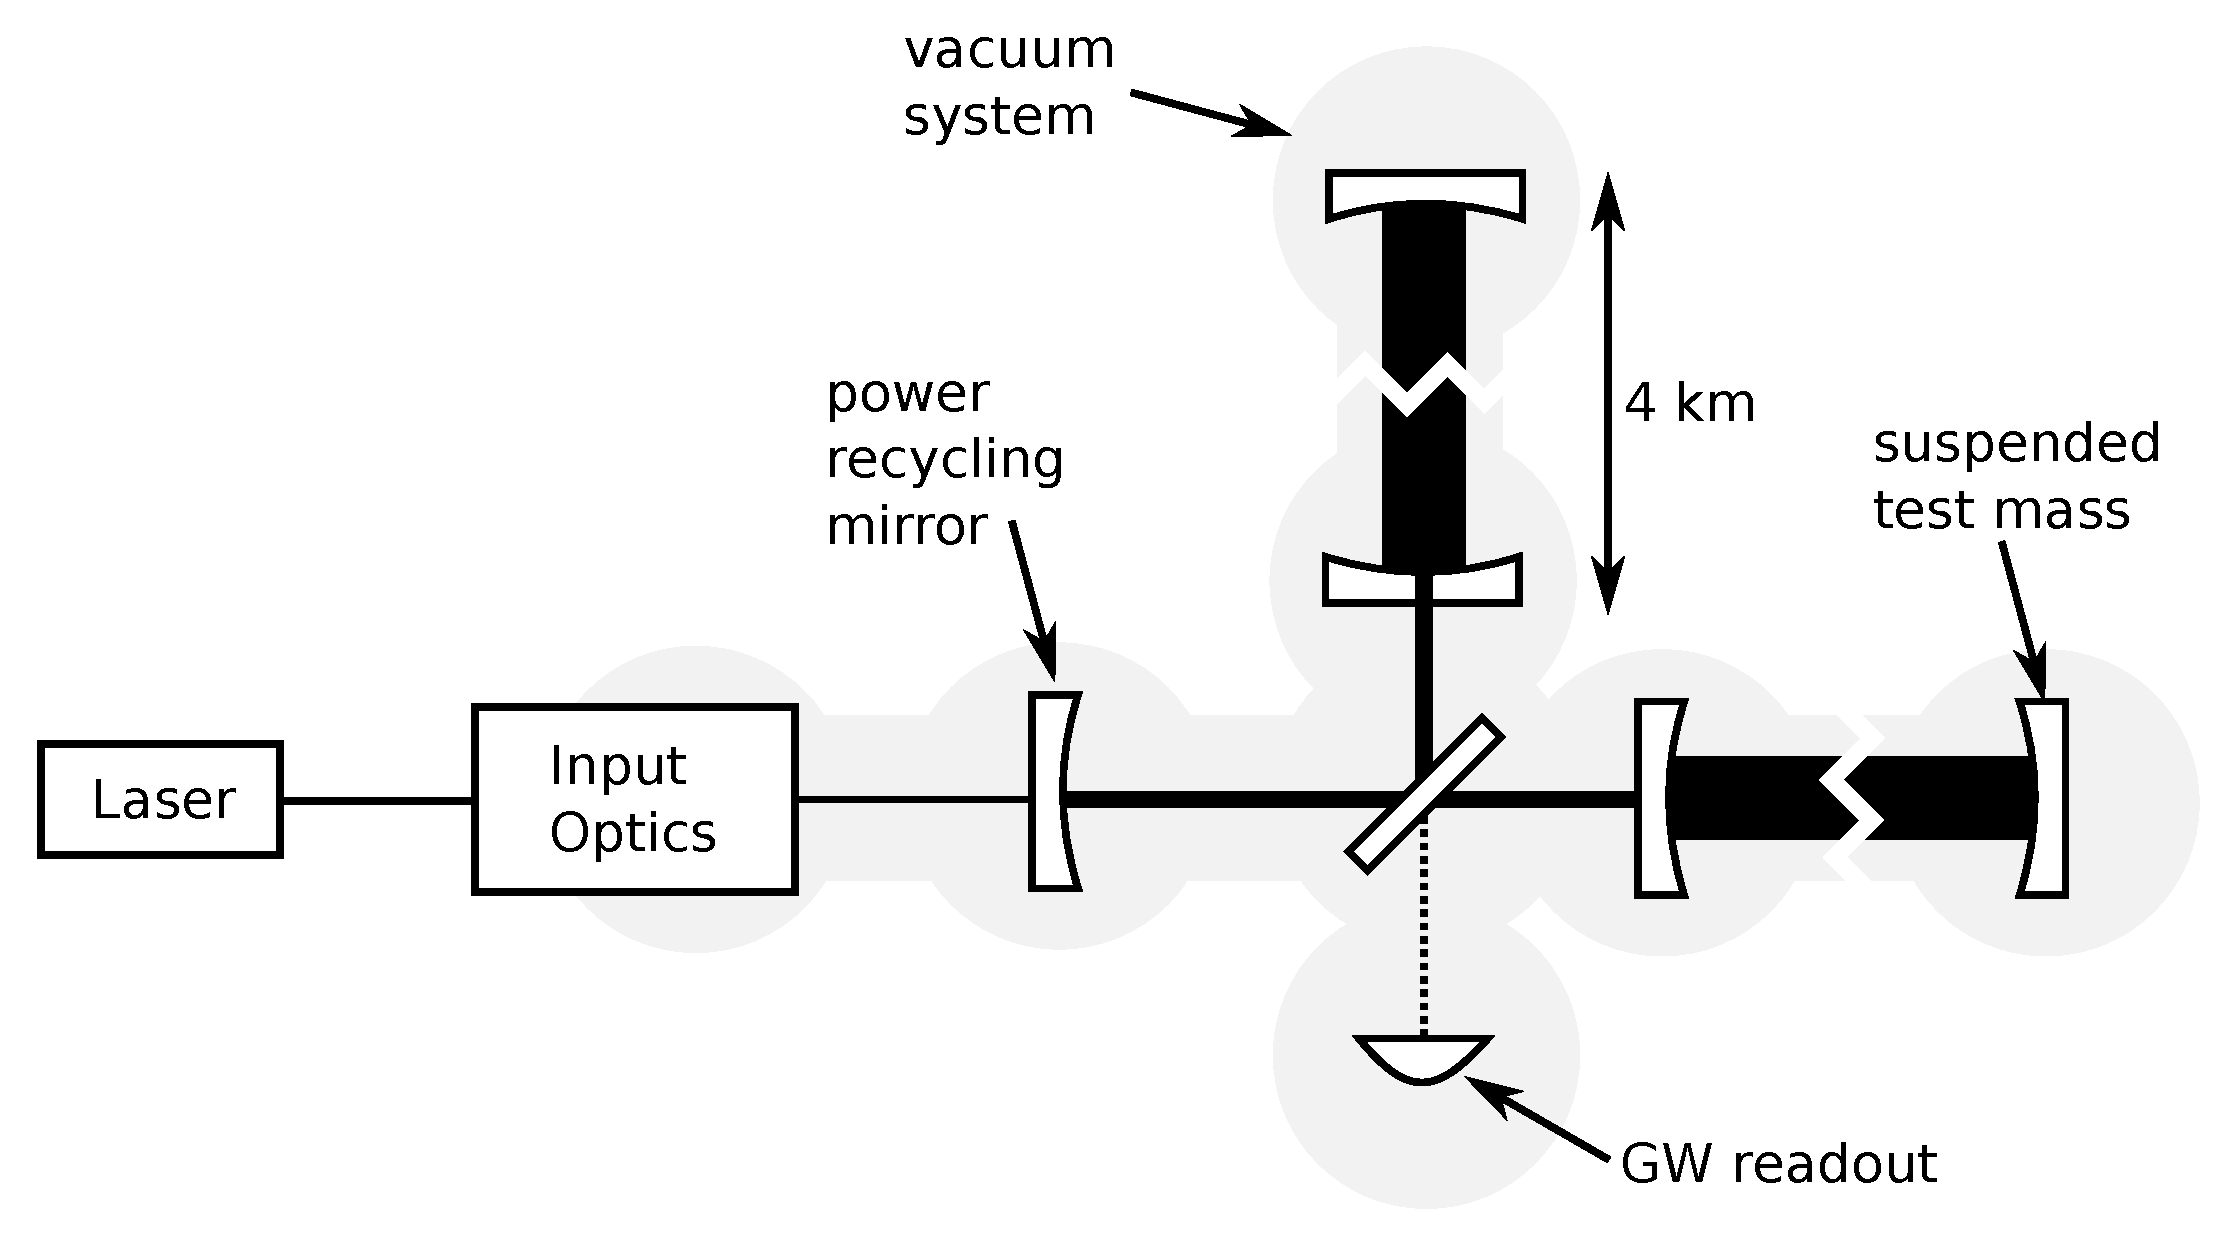
\includegraphics[width=0.8\textwidth]{figures/IFOschematic.pdf}
% \caption[Power-recycled Fabry-Perot Michelson laser
% interferometer]{Power-recycled Fabry-Perot Michelson laser
%   interferometer.}
% \label{fig:IFOschematic}
% \end{centering}
% \end{figure}









\section{Signal Versus Noise}
The factors that must be considered in the design of any detector can
be grouped into two categories: signal and noise. The ability to make
a claim of detection is largely dependent on the magnitude of the
signal to noise ratio (SNR). An SNR of 8 is desired for detection
confidence in LIGO. 

For laser interferometers operating with DC readout, the strength of
the GW signal is proportional to the length of the arms and the amount
of power at the beam splitter. (See Eq. \ref{}.) For a given strain,
the change in the distance between the mirrors, $\Delta L$, is bigger
the longer the arms. And for a given displacement from the dark
fringe, the power that will show up at the AS port is greater the
greater the power at the beam splitter. Therefore, the two fundamental
ways to make a GW produce a bigger signal in an interferometer are:
\begin{enumerate}
\item make the arms longer \vspace{-10 pt}
\item increase the circulating power
\end{enumerate}

No matter how large a signal one might have, it won't be found
confidently, or at all, if there is too much noise. The noise itself
is best grouped into categories of displacement noise and sensing
noise which affect the length of the arms and the measurement of the
signal, respectively. Interferometers for GW detection are plagued
primarily by displacement noise below 70~Hz and sensing noise above
200~Hz.

In the next sections I will describe briefly the specific types of
displacement and sensing noises affecting the sensitivity of laser
interferometers. A summary of the noise budget is shown in
Fig. \ref{fig:NB}. 


\begin{figure}
\begin{centering}
%\includegraphics[width=0.8\textwidth]{figures/.pdf}
\caption[LIGO noise budget]{Noise budget place holder.}
\label{fig:NB}
\end{centering}
\end{figure}


\subsection{Displacement Noise} 
ground motion, thermal noise

seismic noise physically displaces the mirrors, resulting in changes in the length
of the arm. 

\subsection{Sensing Noise}
stray light, shot noise

Shot noise is a quantum mechanical effect of the detection
of photons which creates uncertainty in the phase of the light, and
therefore the power, at the AS port.



\section{fk}
The LIGO interferometers are designed to maximize signal and minimize
noise. The arms are 4~km long, as long as could be made within a
reasonable budget, and we always strive to operate with as much laser
power as is available and practically possible. 


\section{DC readout / more laser power}
Increasing the laser power in the interferometer is a 

Shot noise is a Poissonian process: the average number of photons
striking a detector, $\left<x\right>$, is equal to the variance of the
mean number of photons, $\left<x^2\right> - \left<x\right>^2$, from a
given chunk of time $\tau$ to another. For large $\left<x\right>$, the
distribution becomes Gaussian, but the mean and variance are still
equivalent. Based on this property and Parseval's theorem, the power
on a detector due to shot noise is:
\begin{equation}
P_{SN} = \frac{\left<x\right>}{\tau} h \nu = \sqrt{2 P_{DC} h \nu}
\end{equation}
where $P_{DC}$ is the DC power on the photodiode, $h = 6.626 \times
10^{-34}$ Js is Planck's constant, and $\nu = 2.82 \times 10^{14}$ Hz
is the frequency of the incident light. The units of shot noise are
W/$\sqrt{\mathrm{Hz}}$.

DC readout, as used in Enhanced LIGO, operates with a small offset,
$x_0 \approx 10 \mathrm{pm}$, from the dark fringe. Strain induced in the
interferometer can therefore be directly read out at the dark pork as
simply a linear function of power. We are interested in the optical
gain of this form of readout, the change in power at the AS port per
change in differential arm length. 

The power at the dark port as a function of differential arm length,
$x$, is
\begin{equation}
P_{AS} = P_{BS} \sin^2{(g_{\phi}kx)}
\end{equation}
where $g_{\phi} = 137$ is phase gain of the Fabry-Perot arms and
$k=5.9\times10^6 \mathrm{m}^{-1}$ is the wavenumeber. The derivative
is the optical gain:
\begin{equation}
\frac{dP_{AS}}{dx} = P_{BS} g_{\phi} k \sin{(g_{\phi}kx)} \cos{(g_{\phi}kx)}
\end{equation}

The sensitivity of DC readout to gravitational wave strain is
dependent not only on the optical gain, but on the noise at
detector. The shot-noise-limited sensitivity is the shot noise divided
by the optical gain:
\begin{equation}
aoeu
\end{equation}





\section{Controlling the Interferometer}
The ability of the interferometer to provide a differential arm length
signal depends on the many interferometer cavities being locked
\textcolor{blue}{(define locking!)} all at once. It is the light,
after all, that serves as our probe of arm length. The motion of the
mirrors without any control is too large for a locked state to
naturally occur. The rms pendular displacement of the mirrors without
control is 1 \micron, equivalent to a full laser wavelength. The arm
length would swing from one free spectral range (FSR) to the next,
never staying put long enough at any particular FSR.

The motion of the interferometer mirrors must be controlled enough so
that resonance is achieved and error signals fall in a linear
regime. Since the strain sensitivity is determined by mathematically
undoing the (carefully measured) effect of the control system on DARM,
control does not directly improve the strain sensitivity. The purpose
length control does serves is to make the strain measurement
possible. For other degrees of freedom, such as angular motion, only
the controlled residual matters ..
Control, however, introduces noise so there is a fine
balance that must be found between too much and too little control.

Design considerations for the control loops include how much motion at
what frequencies can be tolerated, and the signal to noise ratio of
the motion sensor.


\subsection{RF Sidebands}
Phase modulation multiplies carrier light with field
$E_0e^{i\omega t}$ by $e^{i \Gamma \sin{(\Omega t)}}$, where $\Gamma$
is the modulation index and $\Omega$ is the frequency of the phase
modulation. Using the Jacobi-Anger expression,
\begin{equation}
e^{i z \sin{\theta}} = \sum_{n=-\infty}^{\infty} J_n(z) e^{i n \theta},
\end{equation}
where $J_n$ are the Bessel functions, we can write the first few terms
(n = 0, 1, -1) of the phase-modulated field:
\begin{equation}
E_{modulated} = E_0 J_0(\Gamma) e^{i\omega t} + E_0 J_1(\Gamma)
e^{i(\omega + \Omega) t} + E_0 J_{-1}(\Gamma)
e^{i(\omega - \Omega) t} + ...
\end{equation}
We see that both an upper and lower primary sideband are created, with
frequencies $\omega + \Omega$ and $\omega - \Omega$. Phase modulation
does produce an infinite number of sidebands, yet the amplitude of the
Bessel function decays rapidly with higher $|n|$, so only this first
set of sidebands are significant.




\subsection{Digital Control in LIGO}
Although the interferometer is an analog instrument, it is interfaced
through a digital control system. The analog sensor signals are sent
through an analog-to-digital converter (ADC), digitally filtered, and
then sent through a digital-to-analog converter (DAC) before returning
to the interferometer's actuators as control signals. The use of a digital
control system means complex filters can be more easily implemented
than they would with analog electronics, and the potential 

There a select few control systems that remain completely analog, like
the laser intensity stabilization servo (ISS). When the frequencies of
interest extend beyond several tens of thousands of Hz, the use of
computers becomes impractical.




\subsection{Mirror Suspension and Actuation}
\label{sec:suspension}
The primary interferometer optics are suspended in vacuum so that they
act like free masses at the frequencies in the GW detection band. Each
mirror is hung from a single \textcolor{blue}{xx m diameter} wire that
loops around the bottom of the barrel of the mirror as shown in
Fig. \ref{fig:suspension}. Stand-offs glued just above the mirror's
center of mass on both sides of the barrel mark the final point of
contact of the wire with the mirror, and both ends of the wire are
clamped to the top of a suspension cage.

Each mirror is equipped with four optical sensor and electro-magnetic
(OSEM) actuators for providing control to the mirror. Magnets arranged
to form the four corners of a square are glued on the mirror's back
surface, and the OSEM units envelop them. Length control of the
cavities, for instance, sends current of the same magnitude through
each coil on a given mirror to provide a piston force for changing the
mirror's position.

Minimal contact with the mirrors is necessary to avoid thermal
noise. Therefore, the suspensions provide minimal damping to the
mirrors. Damping for the large optics is instead achieved
electronically through the use of optical levers. They provide
velocity damping only (no DC control) between 0.2~Hz and 2~Hz. The
open loop transfer function of the optical lever servo is in the
Appendix (Figure~\ref{fig:oplevOLG}).

The suspensions are AC damped at all times for each of the large
optics through optical lever witnesses. Keeping the mirrors quiet
enough with respect to their local ground is necessary to allow for
the initial locking of the interferometer, so each suspended optic,
small and large, is quieted by its OSEM signals during the initial
locking stages. After the interferometer is locked, the angular OSEM
feedback is turned off, and the position OSEM feedback remains.

pitch and yaw

